\documentclass{beamer}
\usepackage{graphicx}
\usepackage[outputdir=./target]{minted}
\usepackage[utf8]{inputenc}

\usetheme{Madrid}
\usecolortheme{dolphin}

\graphicspath{ {images/} }

\title{Degasolv}
\subtitle{A Generic Dependency Resolver}
\author{Daniel Jay Haskin}
\begin{document}
\begin{frame}
  \titlepage
\end{frame}
\begin{frame}
  \centerline{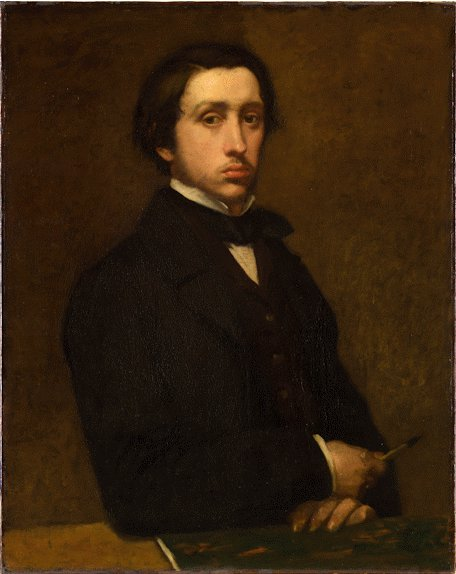
\includegraphics[scale=0.5]{Edgar_Degas_self_portrait_1855.jpeg}}
\end{frame}
\begin{frame}
  \centerline{
\includegraphics[scale=0.15]{DanielHaskin-small.jpg}}
  \center{
    Daniel Jay Haskin \\
    @djhaskin987
  }
\end{frame}
\begin{frame}[fragile]
  \frametitle{Dependencies Are The Worst}

\end{frame}
\begin{frame}
  \frametitle{Why Degasolv?}
  Does this sound like problems you deal with?
  \begin{itemize}
  \item Lots of first party dependencies within the product
  \item All (or lots) of the product's third-party dependencies are built on-site
  \item Some languages/technologies don't have a dependency manager
  \item Cross-technology dependencies
  \item Deal with site-specific quirks
  \end{itemize}
  Then degasolv may be for you.
\end{frame}
\begin{frame}
  \frametitle{Design}
  \begin{itemize}
    \item Degasolv is a ``closed diamond'' resolver
  \end{itemize}
  \centerline{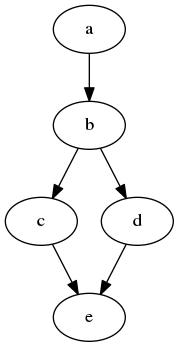
\includegraphics[scale=0.5]{diamonddep.png}}
\end{frame}
\begin{frame}
  \frametitle{Design}
  \begin{itemize}
  \item Degasolv is a ``stays out of your way''
  \item If Degasolv makes you angry, then there is a bug in Degasolv.
  \end{itemize}
  \centerline{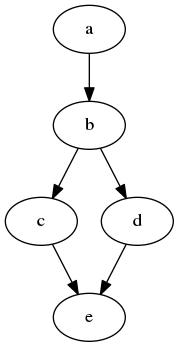
\includegraphics[scale=0.5]{diamonddep.png}}
\end{frame}

\begin{frame}
  \frametitle{Overview}
  \begin{itemize}
  \item \texttt{generate-card}: Generate a ``card file'' which represents a package
  \item Upload the card file to a NAS or other central file share
  \item \texttt{generate-repo-index}: Generate a ``repository index'' based on the card files
    in the central file share
  \item \texttt{query-repo}: Inspect what packages exist in the repository
  \item \texttt{resolve-locations}: Using repository indices, find the locations
    of packages and their dependencies
  \end{itemize}
\end{frame}
\begin{frame}
  \frametitle{What is a Degasolv ``Package''?'}
  \begin{itemize}
  \item A name
  \item A version
  \item A URL
  \item A list of dependencies
  \end{itemize}
\end{frame}
\begin{frame}
  \frametitle{\texttt{generate-card} Overview}
  \begin{itemize}
  \item Degasolv ``stays out of your way''
  \item Generates ``card'' files, which contain data about a particular package
  \item Keeps track of dependency information indepently of actual package file contents
  \item As a convention, it's good to name your dscard file after the file to which \\
    the URL points (e.g., \texttt{e-1.8.0.zip.dscard})
  \end{itemize}
\end{frame}
\begin{frame}[fragile]
  \frametitle{\texttt{generate-card} Example}
\begin{minted}{bash}
    java -jar \
        ./degasolv-1.0.3-SNAPSHOT-standalone.jar \
        generate-card \
        -i "e" \
        -v "1.8.0" \
        -l "https://example.com/repo/e-1.8.0.zip" \
        -C $PWD/e-1.8.0.zip.dscard
\end{minted}
\end{frame}
\begin{frame}[fragile]
  \frametitle{\texttt{generate-card} Output: The \texttt{*.dscard} File}
\begin{minted}{clojure}
    ; Filename: e-1.8.0.dscard
    #degasolv.resolver/PackageInfo
    {
      :id "e",
      :version "1.8.0",
      :location "https://example.com/repo/e-1.8.0.zip",
      :requirements []
    }
\end{minted}
\end{frame}
\begin{frame}[fragile]
  \frametitle{\texttt{generate-card} Final Step: Deposit the Card File}
  \begin{itemize}
  \item After the card file is generated, it needs to be deposited into a \\
    central file share
  \end{itemize}
\begin{minted}{bash}
    $ find .
    .
    ./c-3.5.0.zip.dscard
    ./b-2.3.0.zip.dscard
    ./e-2.1.0.zip.dscard
    ./e-2.4.0.zip.dscard
    ./e-1.8.0.zip.dscard
    ./d-0.8.0.zip.dscard
    ./c-2.4.7.zip.dscard
\end{minted}
\end{frame}
\begin{frame}
  \centerline{\color{blue}\Large \texttt{generate-card} Demo}
\end{frame}
\begin{frame}
  \frametitle{\texttt{generate-repo-index} Overview}
  \begin{itemize}
  \item Patterned after YUM's \texttt{createrepo}
  \item Running \texttt{generate-repo-index} from the directory containing \texttt{*.dscard}
    files.
  \item The index will then contain information about packages represented in those
    files.
  \end{itemize}
\end{frame}
\begin{frame}[fragile]
  \frametitle{\texttt{generate-repo-index} Example}
\begin{minted}{bash}
    java \
        -jar ./degasolv-1.0.3-SNAPSHOT-standalone.jar \
        generate-repo-index \
        -d $PWD \
        -I $PWD/index.dsrepo
\end{minted}
\end{frame}
\begin{frame}[fragile]
  \frametitle{\texttt{generate-repo-index} Output}
\begin{minted}{bash}
    $ find .
    .
    ./c-3.5.0.zip.dscard
    ./b-2.3.0.zip.dscard
    ./e-2.1.0.zip.dscard
    ./e-2.4.0.zip.dscard
    ./e-1.8.0.zip.dscard
    ./d-0.8.0.zip.dscard
    ./c-2.4.7.zip.dscard
    ./index.dsrepo # <----- new file
\end{minted}
\end{frame}
\begin{frame}
  \centerline{\color{blue}\Large \texttt{generate-repo-index} Demo}
\end{frame}

\begin{frame}
  \frametitle{\texttt{resolve-locations} Overview}
\end{frame}
\begin{frame}
  \frametitle{\texttt{resolve-locations} Example}
\end{frame}
\begin{frame}
  \centerline{\color{blue}\Large \texttt{resolve-locations} Demo}
\end{frame}
\begin{frame}
  \frametitle{\texttt{query-repo} Overview}
\end{frame}
\begin{frame}
  \frametitle{\texttt{query-repo} Example}
\end{frame}
\begin{frame}
  \centerline{\color{blue}\Large \texttt{query-repo} Demo}
\end{frame}
\begin{frame}
  % For this demo we will do multi-technology and native in the same demo,
  % Patterned after what I've seen before, but also patterned after the
  % 'Longer Example' I gave in the docs.
  \centerline{\color{blue}\Large Demo}
\end{frame}
\begin{frame}[fragile]
  \frametitle{JFrog CLI Integration}
  \begin{itemize}
  \item JFrog artifactory CLI already pairs well with degasolv
  \end{itemize}
\end{frame}
\begin{frame}[fragile]
\frametitle{JFrog CLI Integration: Setup}
\begin{minted}{bash}
    #!/bin/sh

    package_name="top"
    build_name="jenkins-${package_name}"
    build_number="18"

    jfrog rt build-clean "${build_name}" "${build_number}"
    jfrog rt build-collect-env "${build_name}" "${build_number}"
    jfrog rt build-add-git "${build_name}" "${build_number}"
\end{minted}
\end{frame}
\begin{frame}[fragile]
\frametitle{JFrog CLI Integration: Download}
\begin{minted}{bash}
    for dep in $(java \
        -jar ./degasolv-1.0.3-SNAPSHOT-standalone.jar \
        resolve-locations \
        --repository=<ARTIFACTORY-REPO-URL>/index.dsrepo \
        top_dep_a top_dep_b top_dep_c | \
        awk -F' *@ *' '{print $2}')
    do
        # In this example, the `dep` variable is of the form
        # <artifactory-repo>/<path-to-artifact>
        jfrog rt download \
            --build-name "${build_name}" \
            --build-number "${build_number}" \
            "${dep}"
            ./deps
    done
\end{minted}
\end{frame}
\begin{frame}[fragile]
\frametitle{JFrog CLI Integration: Upload}
\begin{minted}{bash}
    jfrog rt upload \
        --build-name "${build_name}" \
        --build-number "${build_number}" \
        ./target/<artifact> \
        <artifactory-repo>/<path-to-artifact>
    jfrog rt upload \
        --build-name "${build_name}" \
        --build-number "${build_number}" \
        ./target/<artifact>.dscard \
        <artifactory-degasolv-repo>/<path-to-card>.dscard
    jfrog rt build-publish "${build_name}" "${build_number}"

\end{minted}
\end{frame}
\begin{frame}
\frametitle{JFrog CLI Integration: Screenshots}
\end{frame}
\begin{frame}
\frametitle{JFrog CLI Integration: Screenshots}
\end{frame}
\begin{frame}
\frametitle{JFrog CLI Integration: Screenshots}
\end{frame}
\begin{frame}
    \centerline{\color{blue}\Large JFrog CLI Integration Demo}
\end{frame}
\begin{frame}
  \frametitle{Summary}
\end{frame}
\begin{frame}
  \frametitle{Community}
\end{frame}
\begin{frame}
  \frametitle{Future Directions}
  \begin{itemize}
  \item Bintray, Artifactory plugin
  \item Resolution directly from different types of repositories
  \item Homebrew: https://github.com/Homebrew/brew/blob/master/docs/Formula-Cookbook.md
  \item RPM, Debian packages

  \end{itemize}
\end{frame}
\begin{frame}
  \frametitle{Further Reading}
  \begin{itemize}
  \item Kill Your Dependencies http://www.mikeperham.com/2016/02/09/kill-your-dependencies/
  \item Embracing Conway's Law https://wingolog.org/archives/2015/11/09/embracing-conways-law
  \item JFrog Artifactory CLI https://www.jfrog.com/confluence/display/CLI/CLI+for+JFrog+Artifactory
  \end{itemize}
\end{frame}
\begin{frame}
  \centerline{\color{blue}\Large Questions}
\end{frame}
\end{document}
